\chapter{An introduction to asteroseismology}
\label{chap:asteroseismology}

 The field of asteroseismology takes advantage of the pulsations in a star. All stars are different in structure, temperature, radius, luminosity, density and evolution. This is also what separates them from each other in a stellar oscillation spectrum, since it is unique to each type of pulsating star. Some stars oscillates on the pre- ms, others on the ms, and some on the Red Giant Branch. The nature of the oscillation spectra thus allows us to distinguish between stars with different interiors.  
 
Pulsating stars contract and expands periodically, causing brightness changes that can be observed using two methods. 1) Changes in the velocity fields due to the periodic contractions and expansions gives rise to an observable Doppler effect which can be measured using spectroscopy. 2) Periodic brightness and thereby temperature variations causes variations in luminosity which can be measured with photometry. Observations can provide us with oscillation spectra allowing us to extract and identify the nature of each frequency. Modelling the star can then reproduce the environment in the star, specifically the sound speed which changes accordingly with the temperature and chemical compositions. Therefore, comparing these theoretically produced frequencies with observations allows us to estimate the properties in the star.  

\section{Stellar pulsations}

Pulsations in stars is treated three-dimensionally, and assumes a spherical symmetry of the star (which is true when rotation of the star is too small to cause a distortion of the stellar symmetry). The three directions for which the natural oscillation modes have nodes are described by the distance to the center of the star, $r$, co-latitude $\theta$ (measured from pulsation pole) and longitude $\phi$. Nodes are then defined as concentric shells of constant r, cones of constant $\theta$ and finally planes of constant $\theta$. We can then describe the displacement in the ($r$,$\theta$,$\phi$) space as the following

\begin{align}
    & \xi_r(r,\theta,\phi,t) = a(r)Y^{m}_l(\theta,\phi)e^{-i2\pi\nu t}  \\
    & \xi_\Theta(r,\theta,\phi,t) = b(r)\frac{\partial Y^{m}_l(\theta,\phi)}{\partial \theta}e^{-i2\pi\nu t}  \\
    & \xi_\Theta(r,\theta,\phi,t) = \frac{b(r)}{\sin(\theta)}\frac{\partial Y^{m}_l(\theta,\phi)}{\partial \phi}e^{-i2\pi\nu t},
    \footnotemark{}
\end{align}

\noindent where $a(r)$ and $b(r)$ are the amplitudes, $\nu$ is the oscillation frequency (1/Period) and $Y^{m}_l(\theta,\phi)$ are the spherical harmonics given by 

\begin{equation}
    Y^{m}_l(\theta,\phi) = (-1)^{m}\sqrt{\frac{2l+1}{4\pi}\frac{(l-m)!}{(l+m)!}}P^{m}_l(\cos(\theta))e^{im\phi},
\end{equation}

\noindent where $P^{m}_l(\cos(\theta))$ are the Legendre polynomials\footnote{see \citet{aerts2010} for more details.}, with $l$ being the spherical degree and m the azimuthal order \footnotetext{These equations are introduced for the sole purpose of presenting the spherical harmonics. They will not be used for calculations during the project. For more details, see \citep{aerts2010}.}. The normalization constant 
\begin{equation}
    c_{lm} \equiv \sqrt{\frac{2l+1}{4\pi}\frac{(l-m)!}{(l+m)!}},
\end{equation}

\noindent is defined such that the integral over the unit sphere of $|Y^{m}_l|^2 = 1 $. Three quantum numbers describes the modes for 3-D stars, $n$,$l$ and $m$. $n$ is the \textit{radial order} describing the number of radial nodes in the star. $l$ is the \textit{spherical degree} and represents the total number of surface nodes; finally $m$ is the \textit{azimuthal order} where $|m|$ is the number of longitudinal nodes, crossing the equator. It then follows that $l$-$|m|$ are the co-latitudinal nodes. $m$ can vary from $-l$ to $l$, yielding therefore a number of $2l+1$ different nodes for each spherical degree. An example of all geometrical possibilities of an $l=3$ mode can be seen on \figref{l3}. 

\begin{figure}[t]
    \centering
    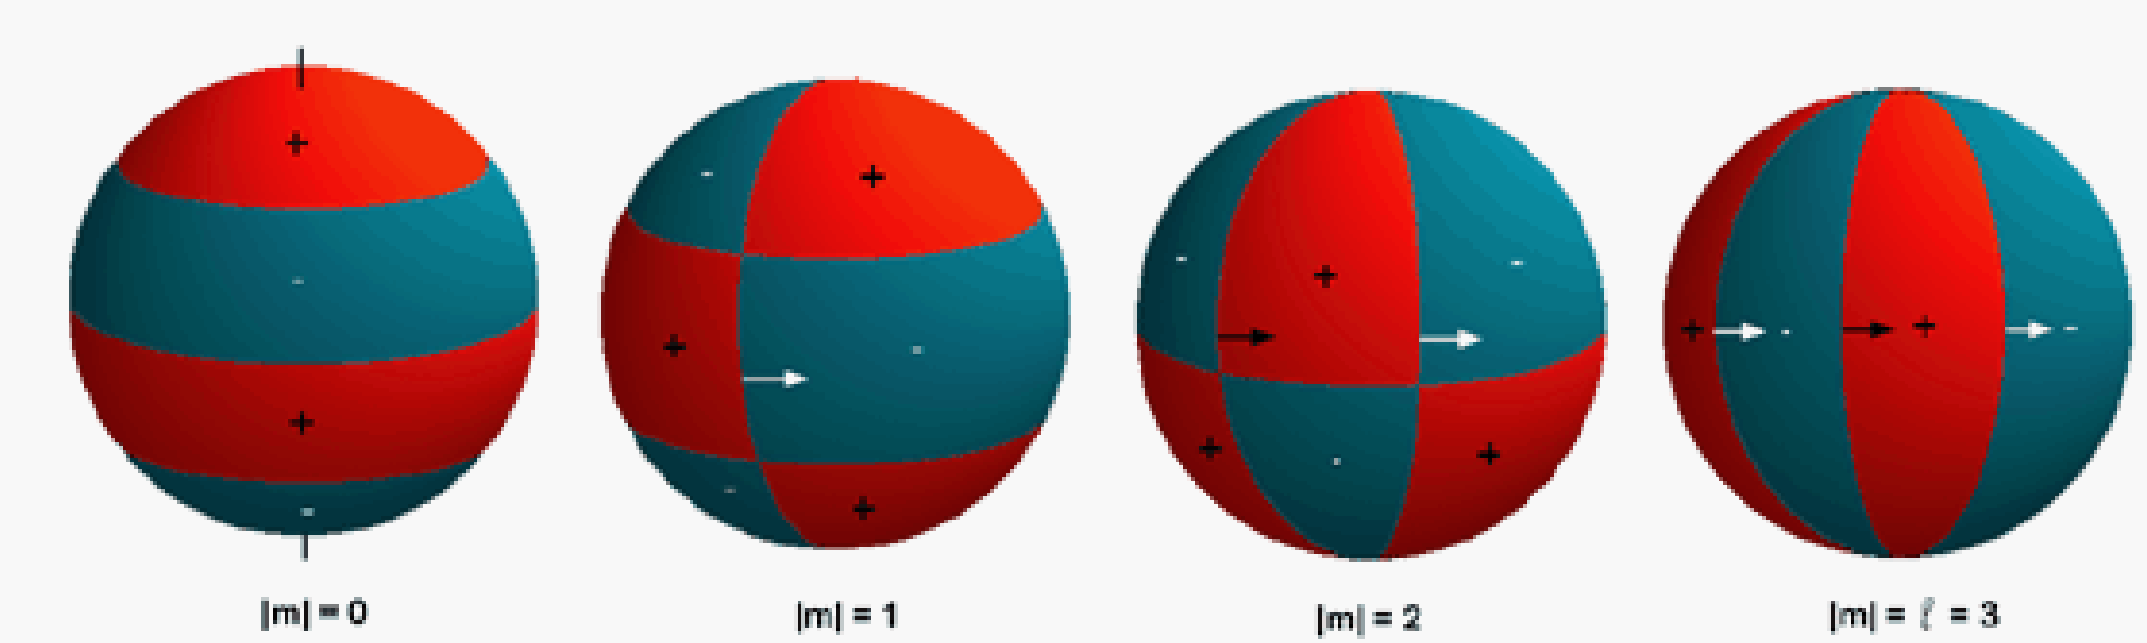
\includegraphics[width=0.8\textwidth]{nonradial.png}
    \caption{Possible geometrical nonradial pulsation patterns with l=3 for a spherically symmetric star. The '+' indicates asreas that moves towards the observer, and the '-' away from the observer. From \citet{antoci2011excitation} (adapted from Wolfgang Zima 1999 master thesis.)}
    \label{l3}
\end{figure}

Generally we can divide stellar pulsations into radial and non-radial pulsations. Radial pulsations is the case for which $l=0$, with the very simplest geometry being the $n=0$\footnote{Note that is also an issue of convention, as some groups prefer the lowest mode to be n=1. This is also the convention used in GYRE (discussed in \chapref{compute})} or \textit{radial fundamental mode}. In this case there is a node only at the center with the corresponding anti-node at the surface, meaning that the entire star pulsates. $n=1$ is the first radial overtone with one node, $n=2$ the second overtone has two radial nodes and so on. %The cases for the radial modes can be seen on \figref{radial}.
If we assume that the star is uniform in temperature and chemical composition we would expect the ratio between the fundamental mode and the first overtone to be similar to that of an organ pipe, see \citet{aerts2010}. However, since we know that the temperature and chemical composition in the star changes with radius, we can exploit the fact that the sound speed changes accordingly, hence affecting the ratio. For instance we expect a ratio of $F/1H = 0.77$ for $\delta Scuti$ stars, but only $F/1H=0.71$ for Cepheids (as they are slightly more evolved). Hence, we can already say something about the interiors based only on two observed frequencies. As for the non-radial modes, the $dipole$ mode is the simplest with $l=1$. They occur only for n>0, e.i there will be at least one radial node in the star in this case. 

As mentioned earlier we have assumed that the star behaves symmetrically, and that for non-radial modes all $|m|$ values have the same frequency as the $|m|=0$. However, if the rotation of a star is fast enough, it can cause the star to deviate from the assumption of spherical symmetry and lift this degeneracy such that all frequencies in $m$ for a given $l$ are different. The Coriolis and centrifugal forces will cause the wave to divert to either slightly lower or higher frequencies. Traveling with the rotation yields the $prograde$ modes (lower frequencies), whereas traveling against rotation are $retrograde$ modes (higher rotation)\footnote{The sign of the quantum number $m$ indicates whether the mode is prograde or retrograde, depending on the convention used.}. Assuming that the rotation still behaves uniformly we can write 

\begin{equation}
    \nu_{nlm} = \nu_{nl0}+ m(1-C_{nl})\Omega/2\pi,
\end{equation}

\noindent where $\nu_{nlm}$ is the frequency, and $\nu_{nl0}$ is the unperturbed central frequency for which $m=0$. The $m=0$ mode is the same even with rotation. $\Omega$ is the angular velocity of the star and finally $C_{nl}$ is the Ledoux constant- calculated from models \citep{aerts2010}, Sec. 2.8. The result from this is that we get a multiplet with $2l+1$ components that \textit{rotationally split} by $(1-C_{nl})\Omega/2\pi$. However, the approximation of a uniform rotation of the star is rather crude. In reality rotation is asymmetric and the rotational splittings depend on several properties of the mode. Also, the components in the multiplet could be excited to different amplitudes or not excited at all. This complicates the identification of the multiplets severely. However, we are nonetheless able to observe these rotational splittings which is very relevant for fast rotating stars. 

\subsection{Pressure and Gravity modes}

Pulsations in stars can generally be divided into two groups: pressure modes (p-modes) and gravity modes (g-modes). The main difference between them is the restoring force in the two cases. I the pressure modes- the pressure is the main restoring force when a star is perturbed from equilibrium, whereas the g-modes have buoyancy as the restoring force. The difference between p-modes and g-modes is depicted on \figref{pandgmodes}, where it can be seen that for p-modes, the gas moves vertically in contrast to the g-modes where the motion is horizontal. It is also possible to observe stars that shows both types of modes i.e. \textit{mixed modes}. There is also a third option between p-modes and g-modes, which are the surface modes or f-modes. These only exist for $l>1$. All three types of modes are shown on \figref{pandgmodes} as a function of spherical degree $l$. 

\begin{figure}[t]
    \centering
    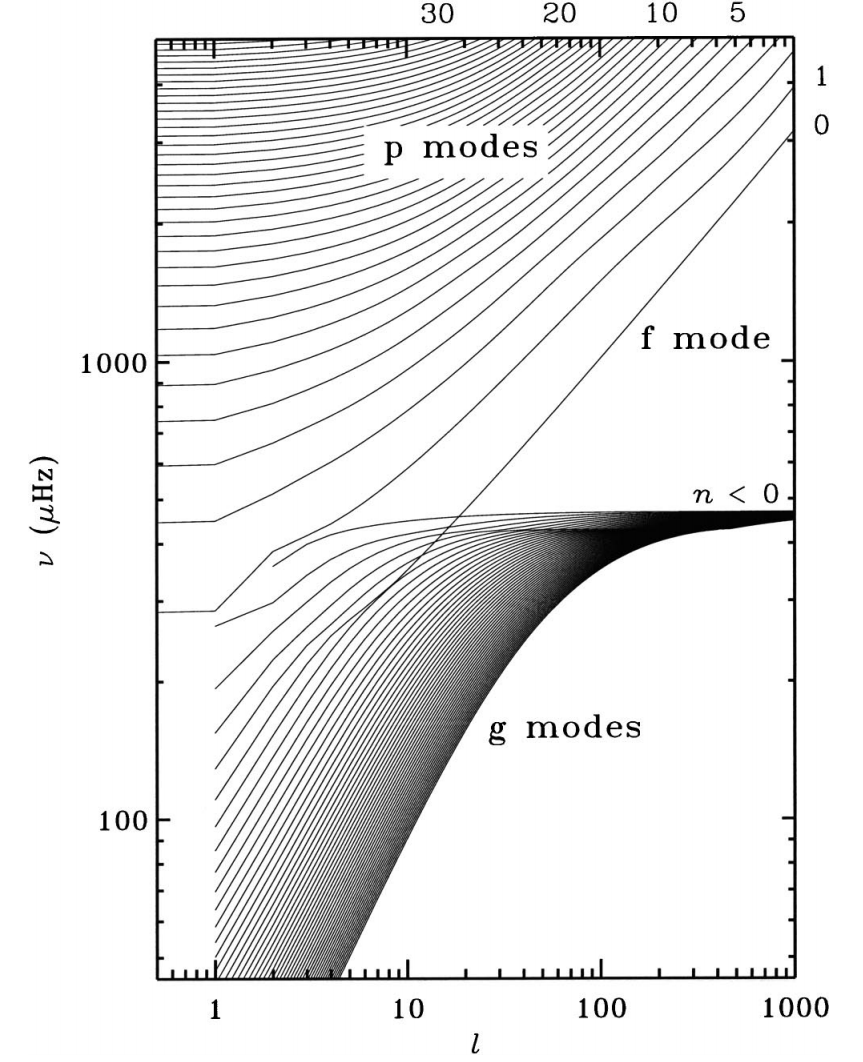
\includegraphics[width=0.6\textwidth]{pandgmodes.png}
    \caption{Frequencies of p and g-modes as a function of spherical degree l for a solar model. For p-modes, the frequency increases with overtone $n$ and spherical degree $l$. For g-modes the it decreases with overtone, although it is a common convention to use negative $n$ for g-modes in which case it will increase. Lines are chosen to illustrate the modes for clarity, but is should be noted that individual modes are discrete points. Figure from \citet{aerts2010}. }
    \label{pandgmodes}
\end{figure}


There are two frequencies that constrains the area in which modes can propagate. The first is the \textit{Lamb frequency}, describing the inverse time needed to travel a horizontal wavelength with local sound speed: 
\begin{equation}
    L_l^{2} = \frac{l(l+1)c^2}{r^2},
\end{equation}

\noindent with l being the spherical degree and c the sound speed at radius r. The second frequency is the \textit{Brunt-Väisälä frequency}. This is the frequency for which a fluent element oscillates around its equilibrium (vertically): 

\begin{equation}
    N^2 = g\left(\frac{1}{H}-\frac{g}{c^2}\right),
\end{equation}

\noindent where H is the density scale height and g is the local gravity.
Together these frequencies define cavities where a mode can oscillate: 

\begin{itemize}
    \item $\omega^2 > L_l^2$ and $\omega^2 > N^2$ where $\omega$ is the eigenfrequency mode. This region is situated in the outer layers of the star where the restoring force is pressure. Hence, oscillations in this area are the p modes. 
    \item $\omega^2 < L^2_l$ and $\omega^2 < N^2$ is the cavity for which the restoring force is buoyancy, hence pulsation modes propagates as g modes. 
\end{itemize}

Energy from modes are mainly distributed to the layers whereas a pulsation can propagate, wheres outside the cavities the mode is damped or \textit{evanescent}. The Brunt-Väisälä and Lamb frequency region is depicted in \figref{pandg} for a post main-sequence 1.9\msun model. Left panels show the propagation diagram for three different stages of the star that are depicted on the evolutionary track on the right panels. In the propagation diagram the dimensionless frequency is plotted as a function of the fractional radius. The p-modes are located towards the surface of the star, with the cavity marked off with the red line. The cavity for g-modes is marked as a black line and peaks towards the center of the star.
\begin{figure}
	\centering
	\begin{subfigure}[b]{1\textwidth}
		\centering
		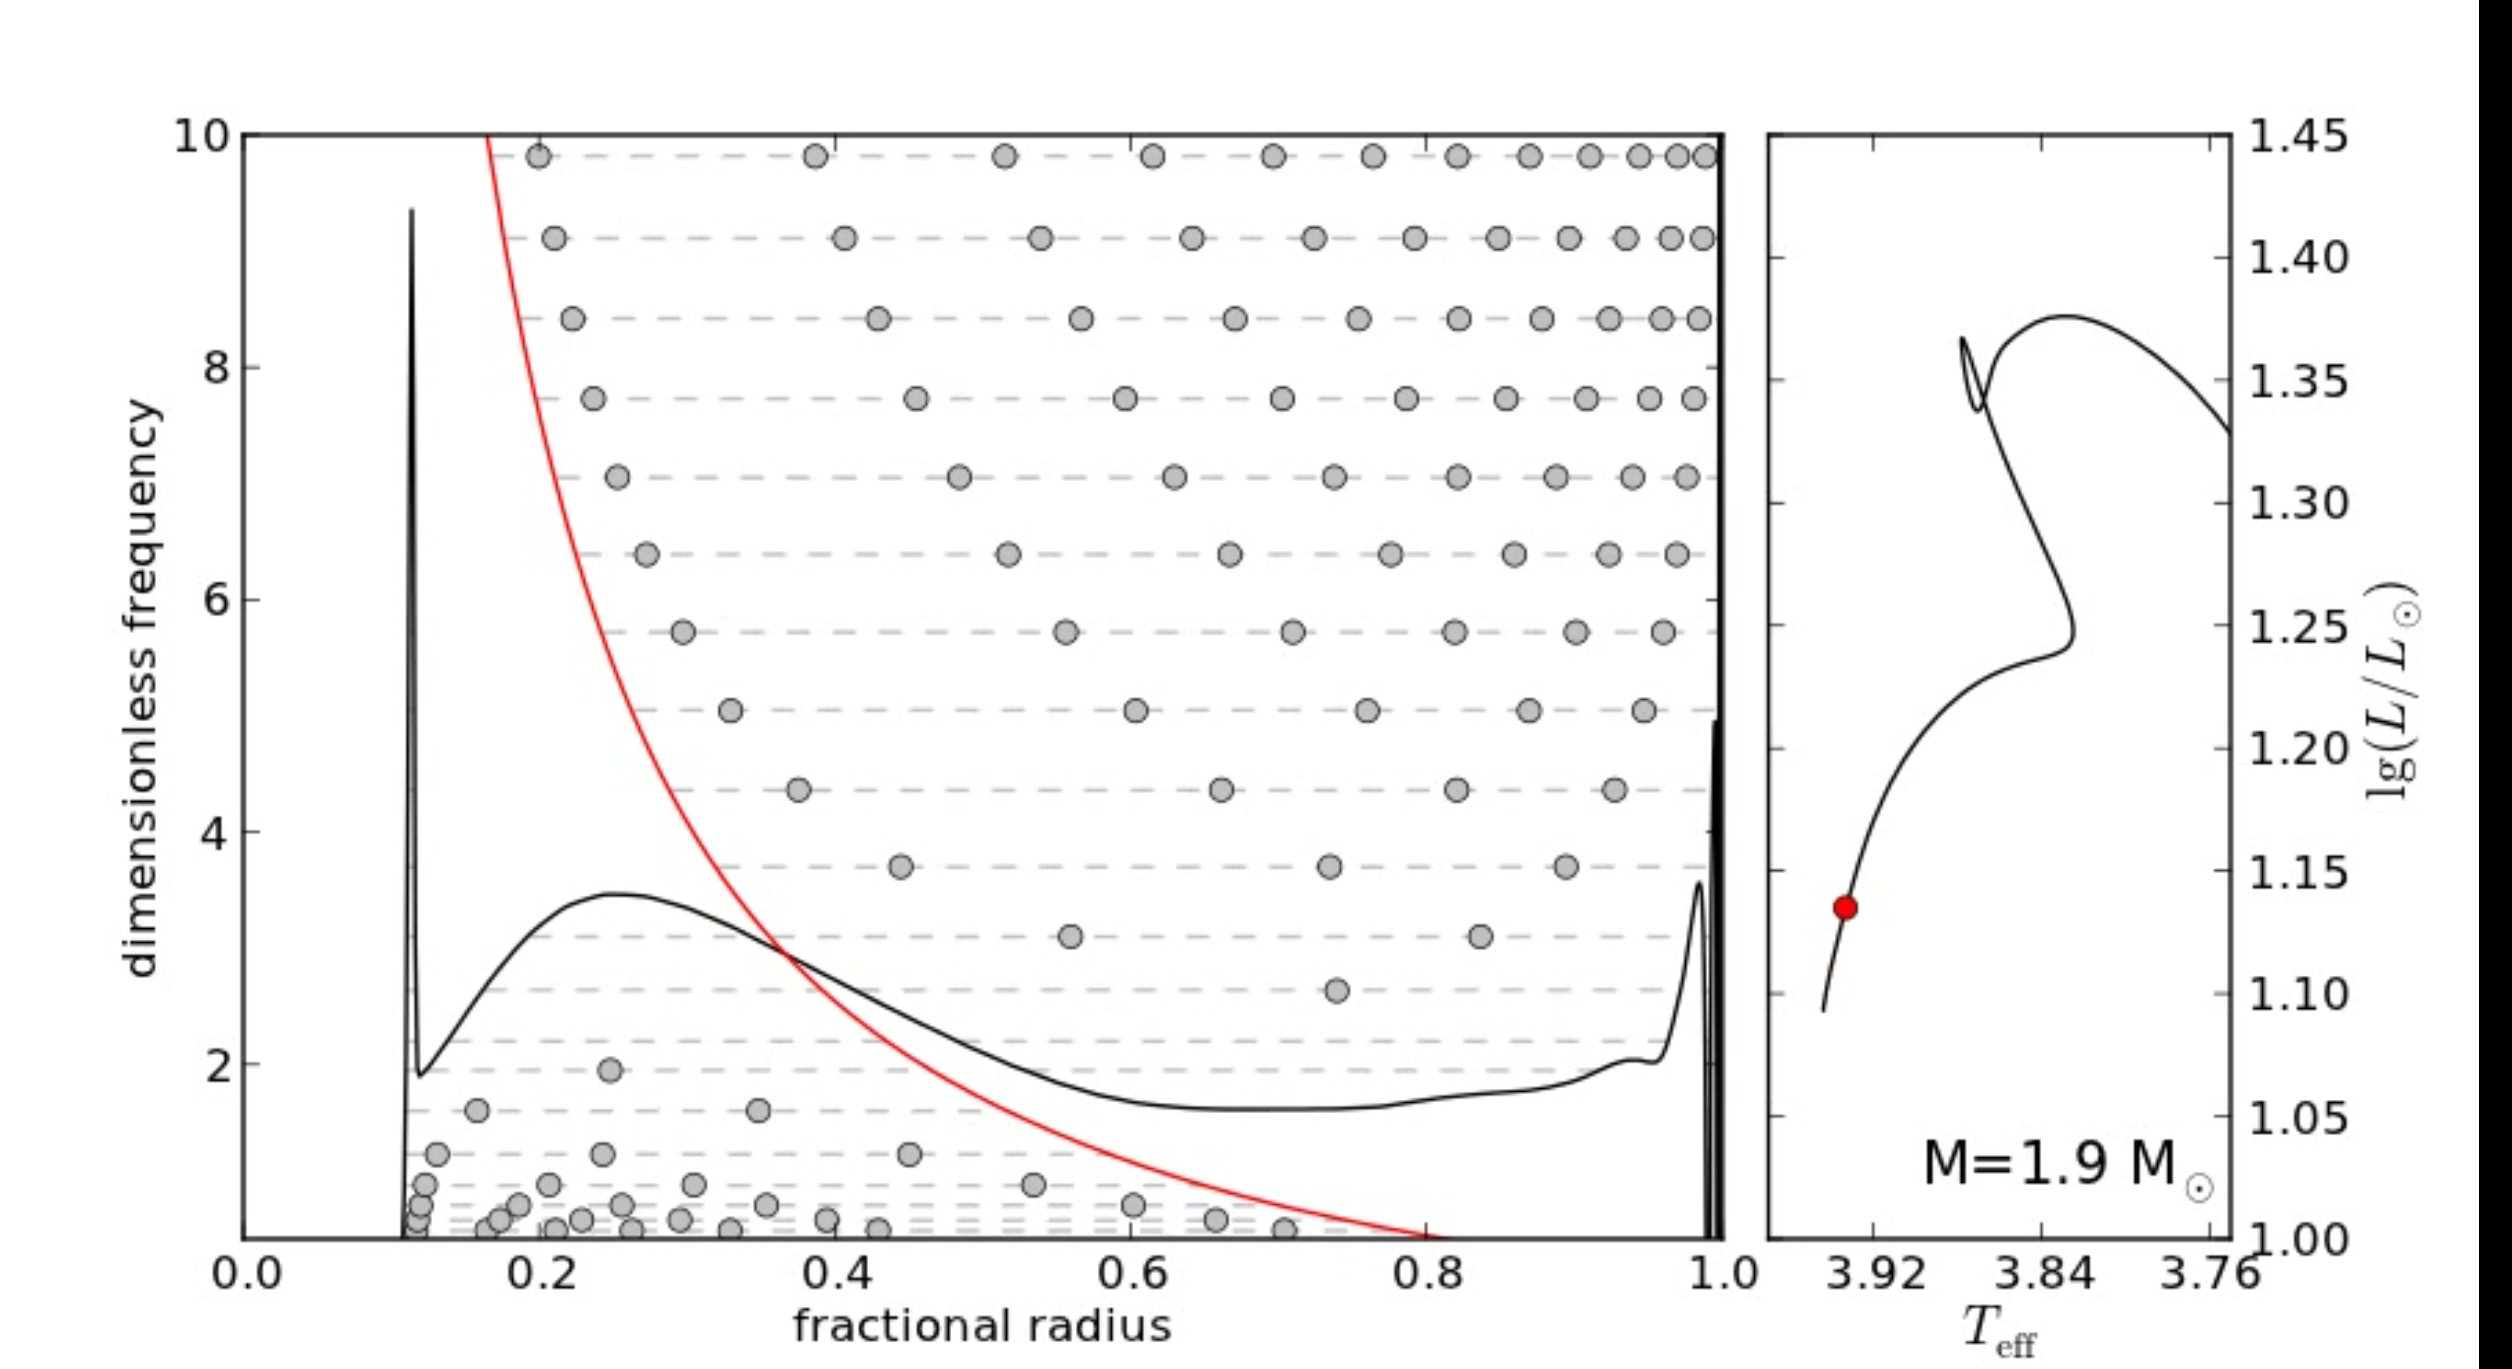
\includegraphics[width=0.9\textwidth, trim={3cm 1.3 1.2cm 1},clip]{propagation1.png}
		\caption{Frequencies of p- and g-modes on the ms. }
		\label{fig:y equals x}
	\end{subfigure}
	\hfill
	\begin{subfigure}[b]{1\textwidth}
		\centering
		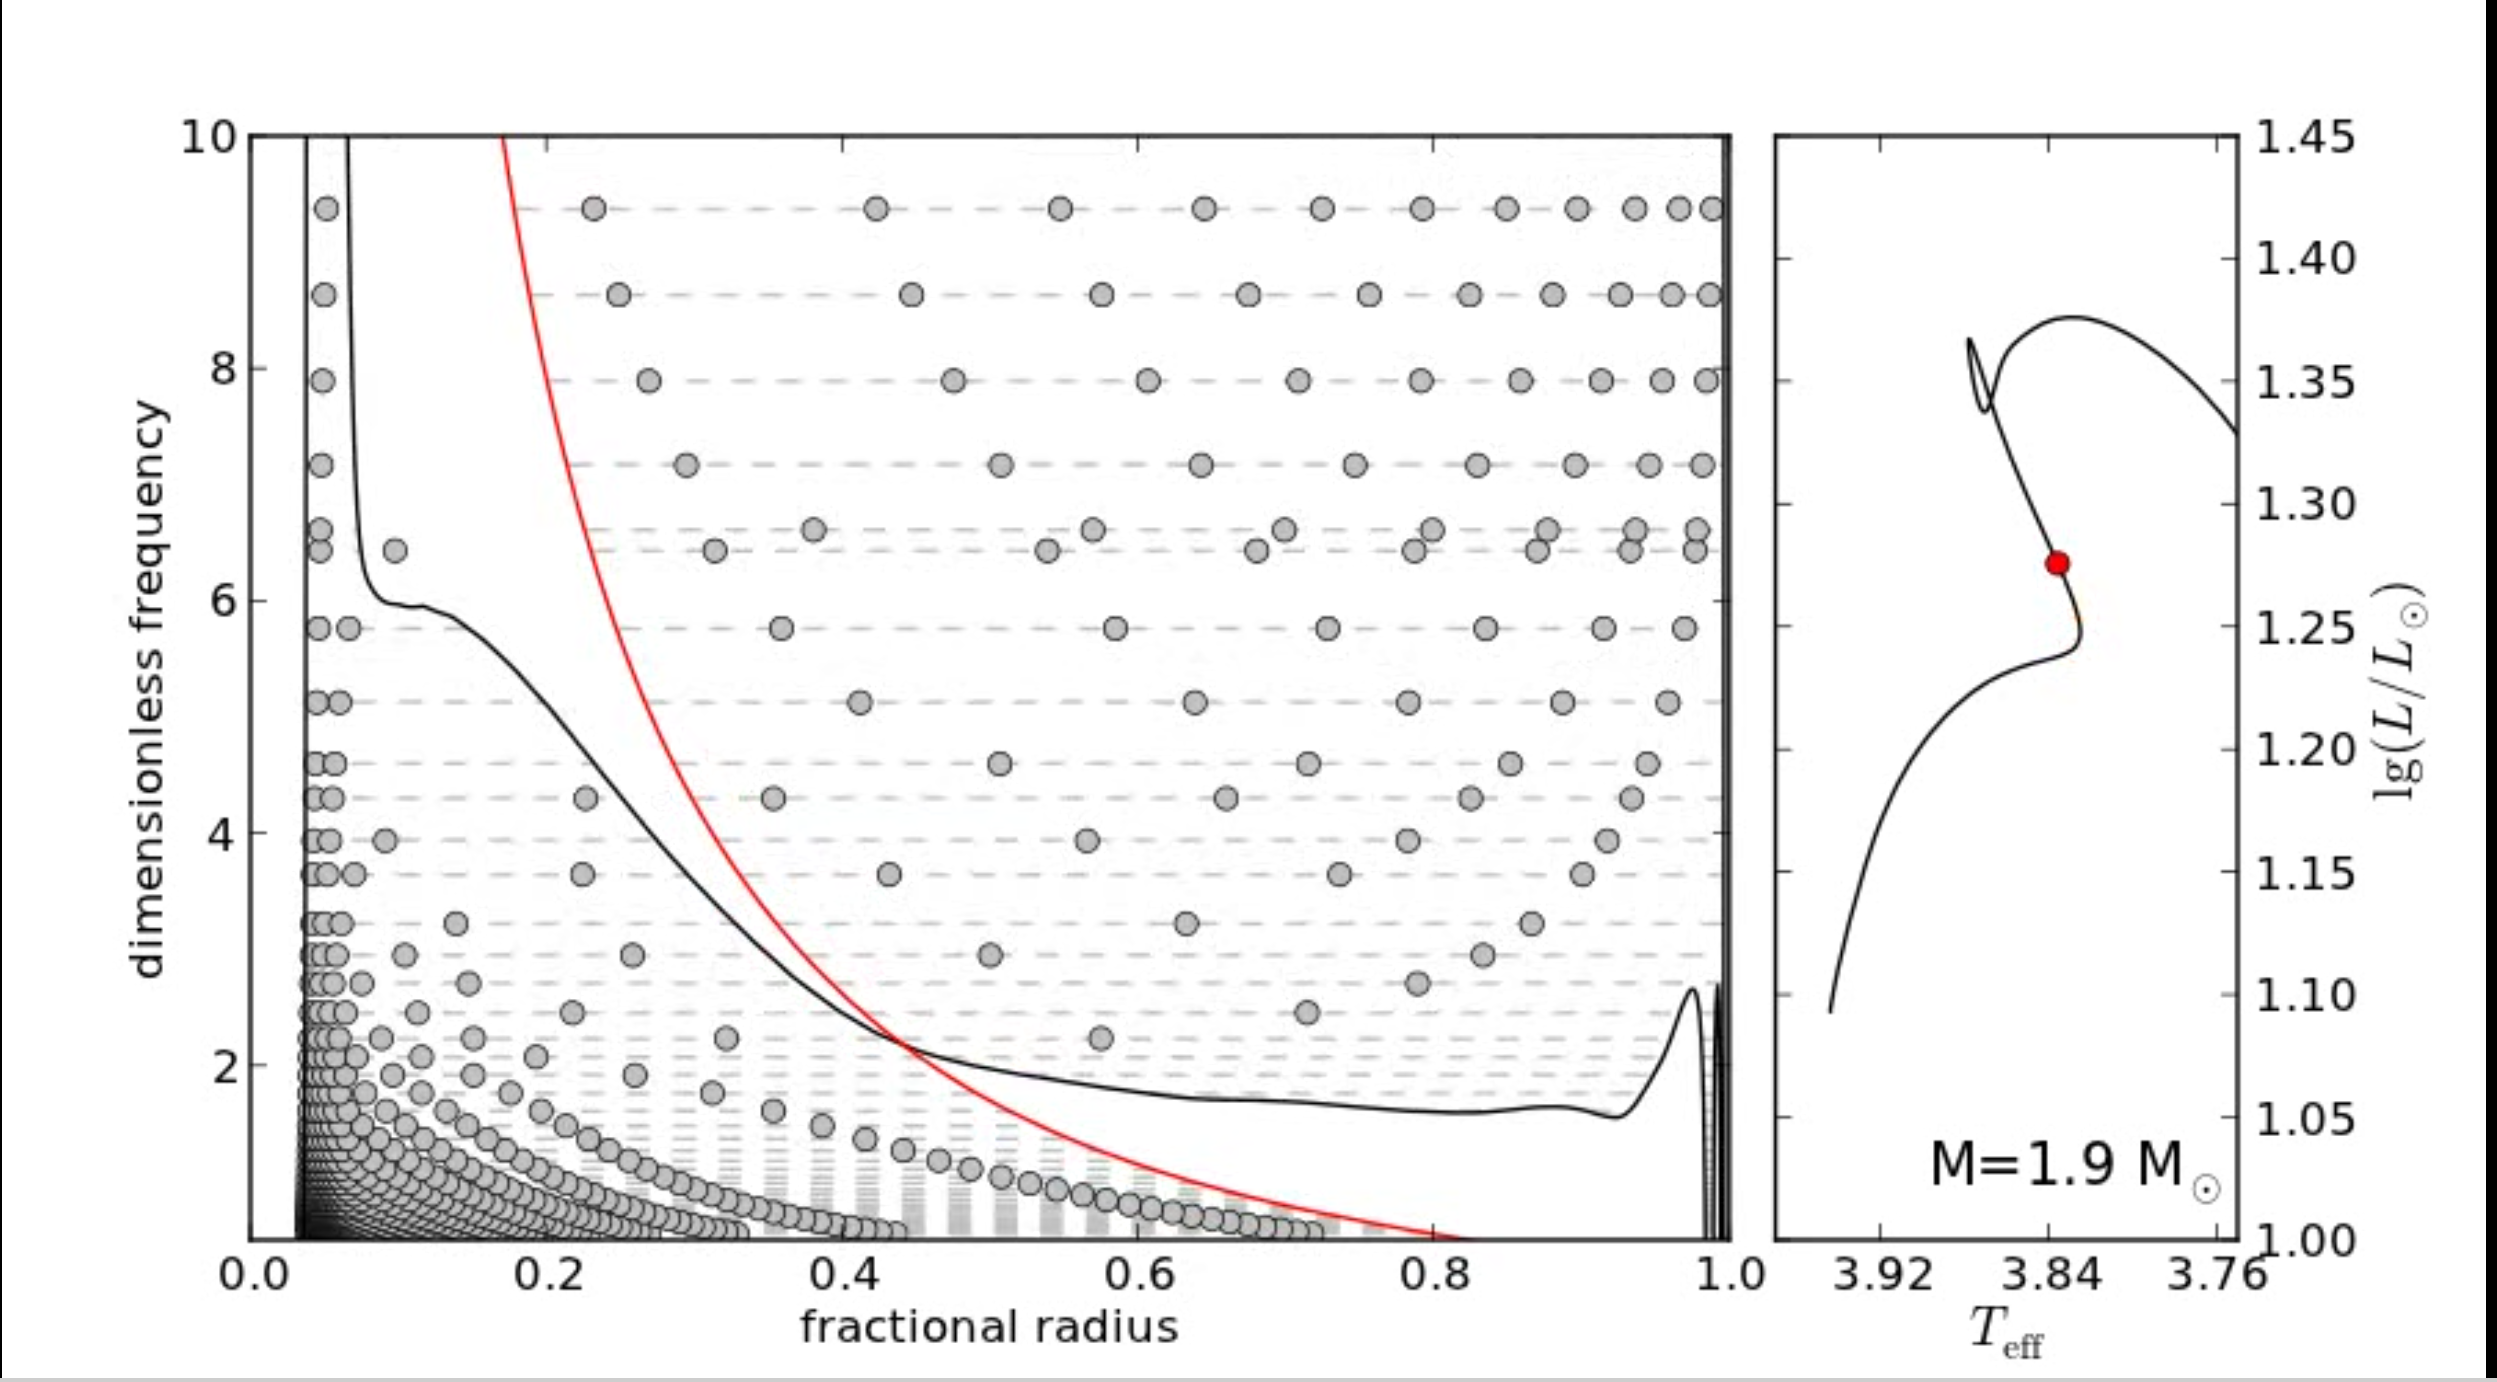
\includegraphics[width=0.9\textwidth,trim={3cm 1.3 1.2cm 1},clip]{propagation2.png}
		\caption{Frequencies of p- and g-modes on the post-0ms contraction phase. }
		\label{fig:three sin x}
	\end{subfigure}
	\hfill
	\begin{subfigure}[b]{1\textwidth}
		\centering
		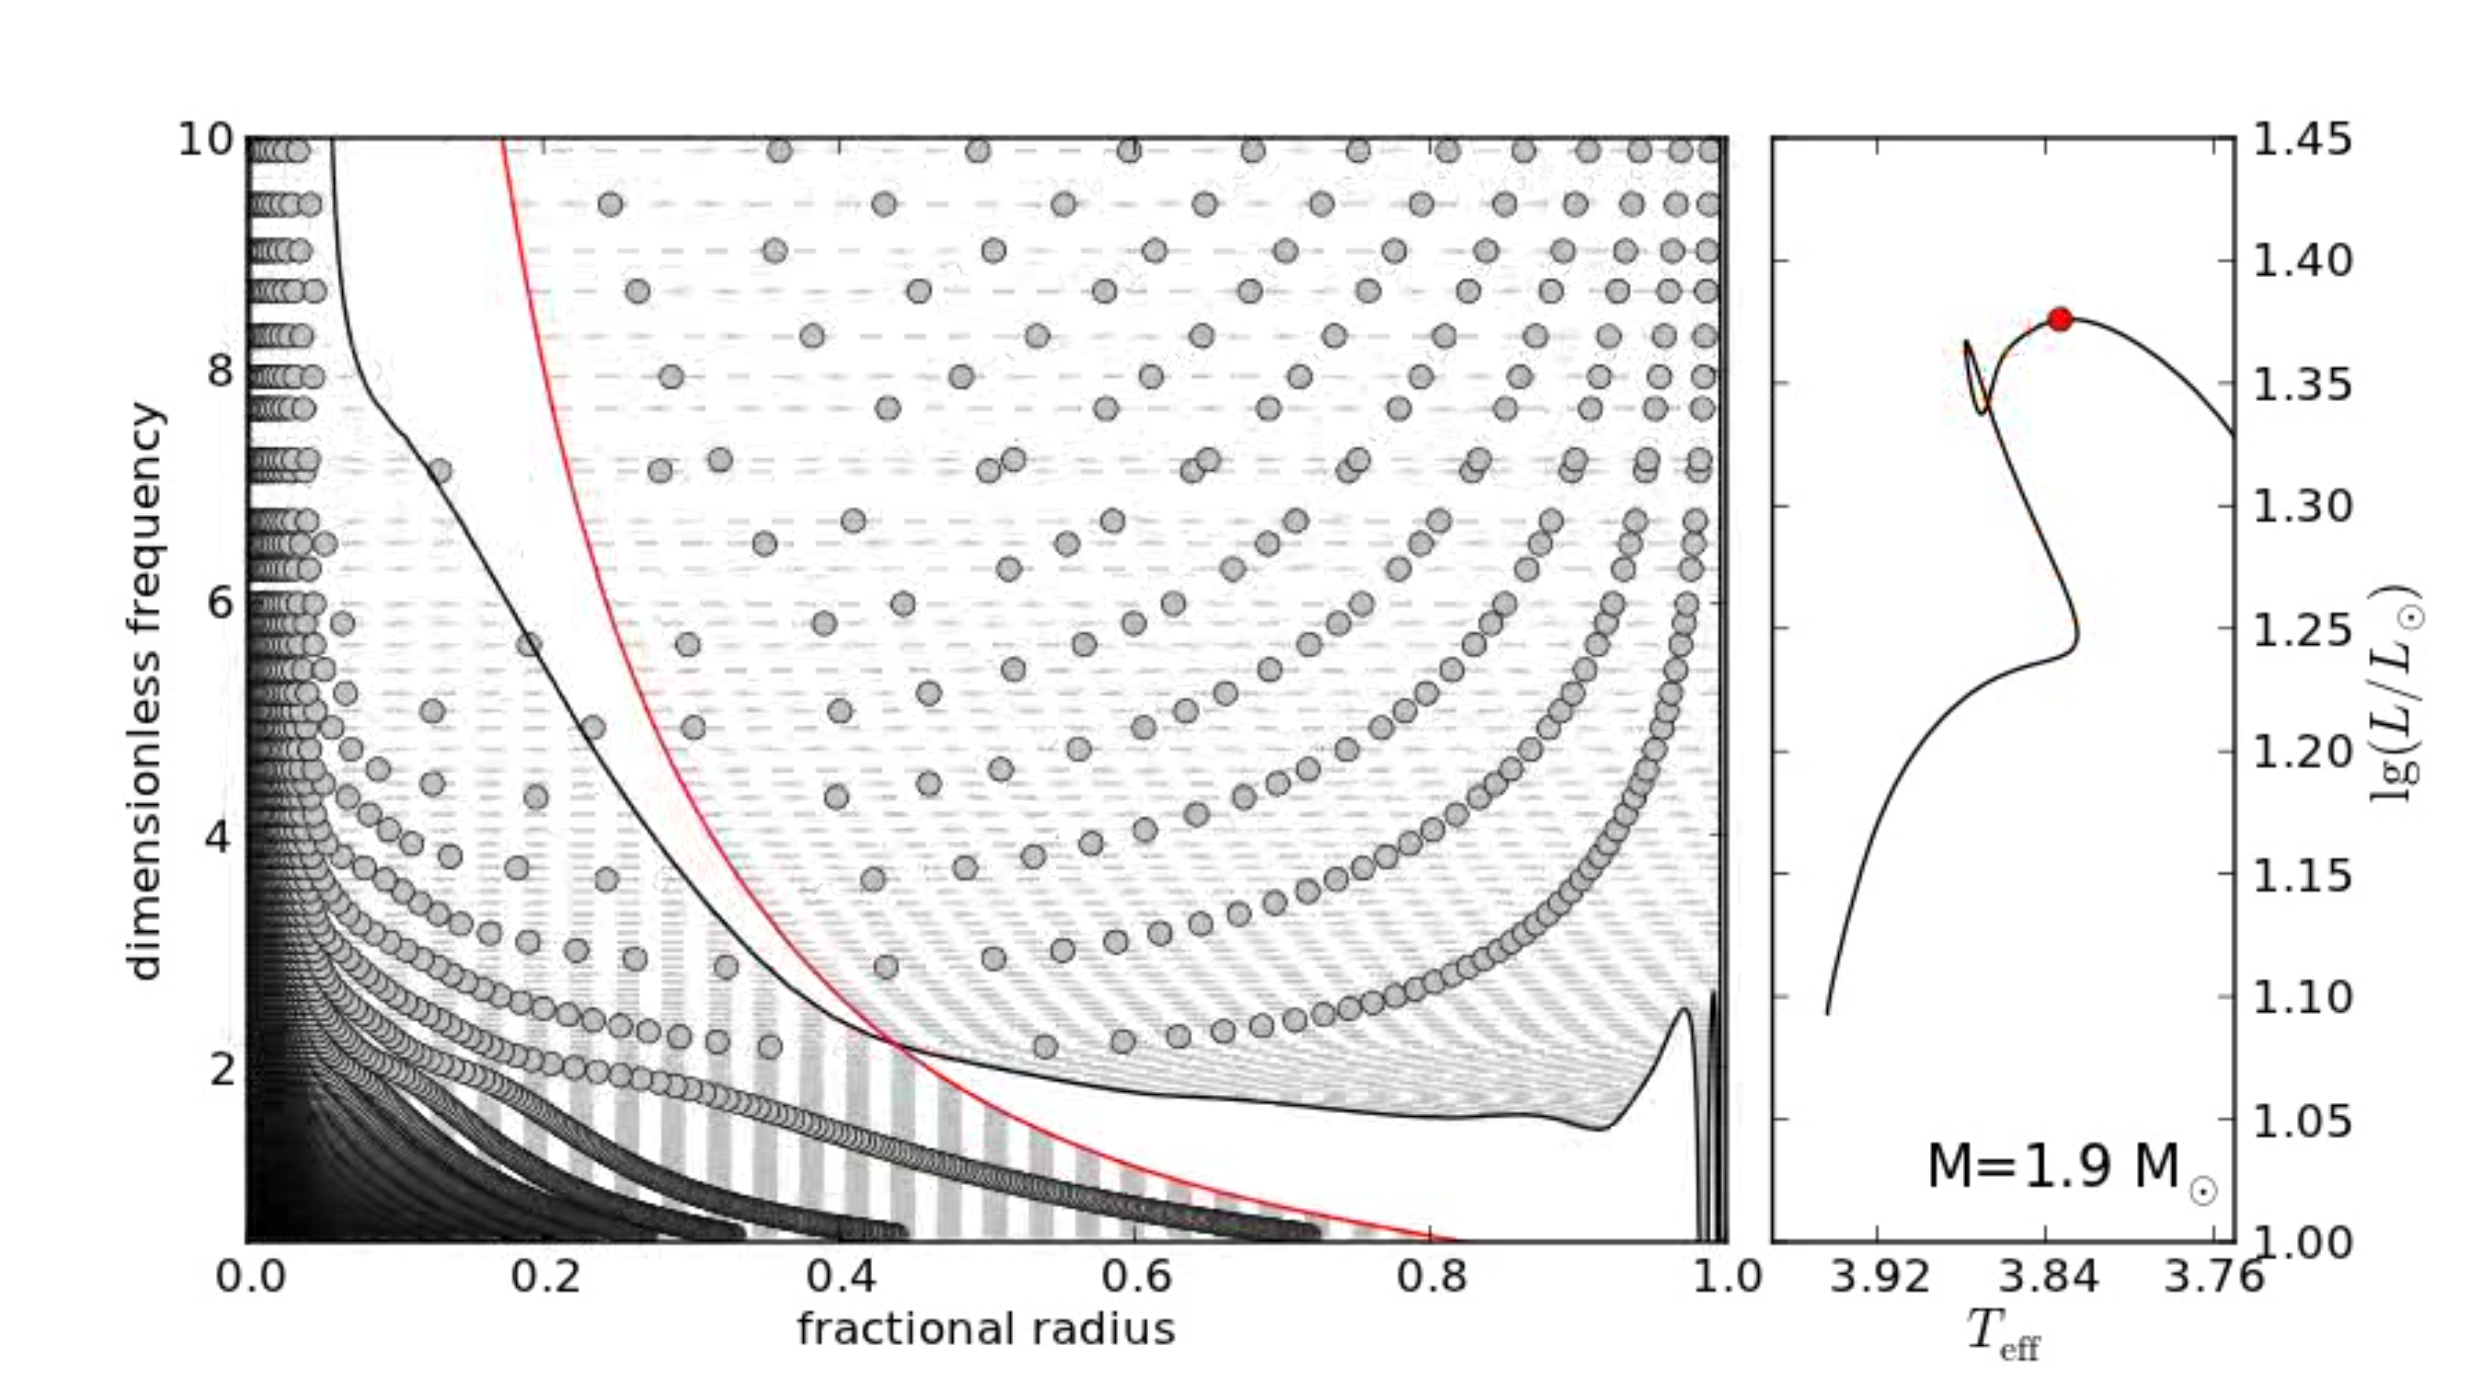
\includegraphics[width=0.9\textwidth,trim={3cm 1.3 1.2cm 1},clip]{propagation3.png}
		\caption{Frequencies of p- and g-modes on the post-ms expansion phase. }
		\label{fig:five over x}
	\end{subfigure}
	\caption{ Left panels shows the propagation diagrams of p and g modes in a 1.9 \msun star as a function fractional radius (0.0 being the center). Right panels shows the evolutionary track for the corresponding propagation diagram, with the current stage marked with a black dot. Credit Patrick Lenz.  }
	\label{pandg}
\end{figure}


Mixed modes exists in the overlapping area of the p-mode and g-mode cavities. They act as g-modes in the interior and p-modes in the outer layers. As the star becomes more evolved the modes change:

\begin{itemize}
	\item There is a  general increase in both p-modes and g-modes. 
	\item The spacing between frequencies decreases as the star becomes more evolved.
	\item The cavity for g-modes grows in frequency and radius space. I.e. more evolved stars have more g-modes.
	\item The g-mode cavity will overlap the p-mode cavity more in evolved stars resulting in an increasing number of mixed modes.  
\end{itemize}

Since the frequencies in a star depends very strongly on the environment,i.e structure, they can therefore act as a tracer for the evolutionary stage of the star. 
 
We can also exploit that different pulsation modes penetrates different layers of the stars. The depth which a mode will penetrate into is determined by the spherical degree l. \figref{rays} shows that the different \textit{ray paths} for different spherical degrees. Dashed lines indicate the turning point where the wave front will be diverted back to the surface. Here, the mode frequency is equal to the local Lamb frequency. The wave is then reflected backwards again due to the drop in density in the outer layers. Besides from p-modes being more sensitive to conditions in the outer layers and for g-modes in the interior layers, there are two other important properties for p-modes and g-modes: 1) As the number of radial nodes increase, so will the frequencies of the p-modes, whereas the frequencies for g-modes will decrease. 2) for $n\gg l$ there is an asymptotic relation for p-modes. This states that the modes are equally spaced in frequency. A similar relation exists for g-modes, however stating that modes are equally spaced in period. 

\begin{figure}[t]
    \centering
    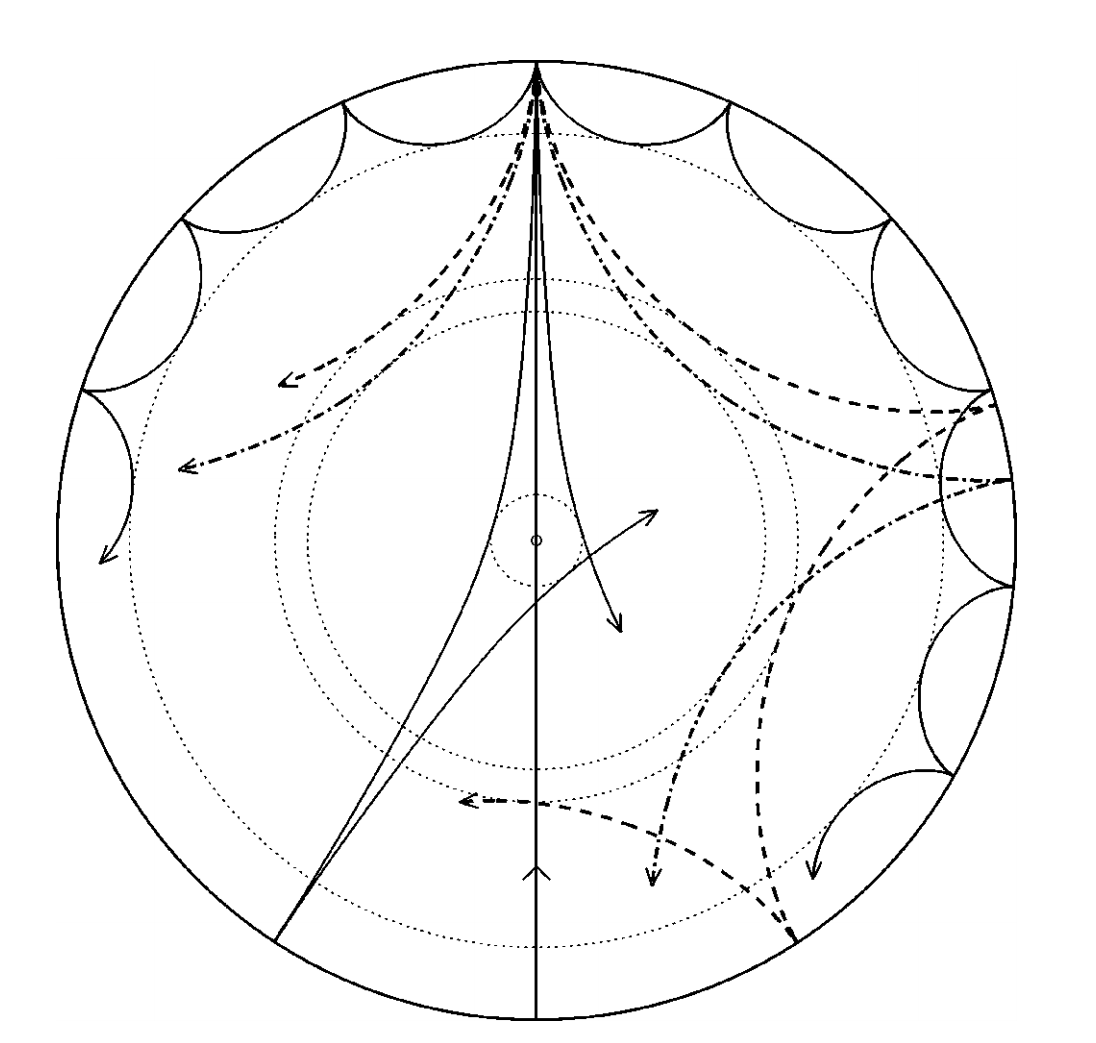
\includegraphics[width=0.8\textwidth]{propagationrays.png}
    \caption{Schematic view of the propagating p-modes in a star. The rays penetrate the star to a depth depending  on the spherical degree, $l$. The ray reaches an point where it will turn around. This is due to the increasing sound speed with depth. After the turnaround, the star will eventually be reflected near the surface, due to a fast decrease in density. The straight line shows the acoustic ray paths of $l$= 0 , 2,20,25 and 7. From J. Christensen-Dalsgaard, 1997, the Theoretical Astrophysical Centre, Institute of Physics and Astronomy, Aarhus University.}
    \label{rays}
\end{figure}

\citep{tassoul1980, tassoul1990} used asymptotic theory to calculate the frequencies of p-modes as the following: 

\begin{equation}
    \nu_{n,l} = \Delta\nu\left(n+\frac{l}{2}+\widetilde{\alpha}\right) + \epsilon_{n,l},
\end{equation}

\noindent where $n$ and $l$ are the radial order and the spherical degree of the mode, $\widetilde{\alpha}$ is a constant of order unity, $\epsilon_{n,l}$ is a small correction and finally $\Delta\nu$ is \textit{the large frequency separation}. This is the inverse of the sound travel time traveling from the surface to the core and back. It is given by: 

\begin{equation}
    \Delta\nu = \left( 2\int_{0}^{R}\frac{dr}{c(r)}\right)^{-1}
\end{equation}

\noindent where $c(r)$ is the sound speed. It can be seen from this that this separation is sensitive to the radius of the star, and is thus a measure of the mean density. 

The asymptotic relation for g-modes states that the periods of g-modes are given by: 

\begin{equation}
    \Pi_{n,l} = \frac{\Pi_0}{\sqrt{l(l+1)}}(n+\epsilon),
\end{equation}

\noindent where $n$ and $l$ are radial order and spherical degree, $\epsilon$ is a small constant and 

\begin{equation}
    \Pi_{0} = 2\pi^2\left(\int \frac{N}{r} dr\right)^{-1},
\end{equation}

\noindent where N is the Brunt-Väisälä frequency and the integral is over a cavity in which a given g-mode propagates.

